\section{Problem No.2} \label{sec:prob2}
\subsection{Problem Description:} 
The FirzHugh-Nagumo equations 
$$
\frac{\partial v}{\partial t} = D\Delta v + (a-v)(v-1)v - w+I
\\
\frac{\partial w}{\partial t} = \epsilon (v-\gamma w)
$$
are used in electrophysiology to model the cross membrane electrical potential (voltage) in cardiac tissue and in neurons. Assuming that the spatial coupling is local and passive results the term which looks like the diffusion of voltage. The state variable are the voltage $v$ and recovery variable $w$.
\begin{enumerate}
\item Write a program to solve the FirzHugh-Nagumo equation on the unit square with homogeneous Neumann boundary conditions for $v$ (meaning electrically insulated). Use a fractional step method to handle the diffusion and reactions separately. Use an ADI method for diffusion solve. Describe what ODE solver you used for the reactions and what fractional stepping you chose. 
\item Use the following parameters $a=0.1, \gamma =2, \epsilon=0.005, I=0, D=5\times 10^{-5}$, and initial conditions 
$$
v(x,y,0)=exp(-100(x^{2}+y^{2}))
\\
w(x,y,0)=0.0
$$
Note that $v=0, w=0$ is a stable steady state of the system. Call this the rest state. For these initial conditions the voltage has been raised above in the bottom corner of the domain. Generate a numerical solution up to time $t=300$. Visualize the voltage and describe the solution. Pick space and time steps to resolve the spatiotemporal dynamics of the solution you see. Discuss what the grid size and time step you used and why. 
\item Use the same parameters from part (2), but use the initial conditions 
$$
v(x,y,0) = 1-2x
\\
w(x,y,0) = 0.05y
$$
and run the simulation until time t=600. Show the voltage at several points in time (pseudocolor plot, contour plot, or surface plot $z=V(x,y,t)$) and describe the solution. 
\end{enumerate}
\subsection{Solution:}
\paragraph{Part 1 \& 2:} 
FirzHugh-Nagumo equations can be solved using Strang splitting (second order accurate) such that the diffusion part is solved using ADI with time step $\Delta t$ and the reaction part along with the second equation is solved using time steps of $\Delta t$. We start by solving the the reaction and the second equation which produce a non-linear coupled system of ODE which can be solved using RK4. We can write the equations as follows 
$$
\frac{dv}{dt}= f_{v}(v,w) =(a-v)(v-1)v - w + I
\\
\frac{dw}{dt}= f_{w}(v,w) =\epsilon (v-\gamma w)
$$
The RK4 solver of this system is 
$$
v^{n+1} = v^{n} + \frac{1}{6}(kv_{1}+2kv_{2} + 2kv_{3}+kv_{4}), \qquad
w^{n+1} = w^{n} + \frac{1}{6}(kw_{1}+2kw_{2} + 2kw_{3}+kw_{4})
\\
kv_{1} = \frac{\Delta t}{2}f_{v}(v,w), \qquad\qquad\qquad\qquad\qquad\qquad
kw_{1} = \frac{\Delta t}{2}f_{w}(v,w)
\\
kv_{2} = \frac{\Delta t}{2}f_{v}(v+\frac{1}{2}kv_{1},w+\frac{1}{2}kw_{1}), \quad\qquad\qquad
kw_{2} = \frac{\Delta t}{2}f_{w}(v+\frac{1}{2}kv_{1},w+\frac{1}{2}kw_{1})
\\
kv_{3} = \frac{\Delta t}{2}f_{v}(v+\frac{1}{2}kv_{2},w+\frac{1}{2}kw_{2}), \quad\qquad\qquad
kw_{3} = \frac{\Delta t}{2}f_{w}(v+\frac{1}{2}kv_{2},w+\frac{1}{2}kw_{2})
\\
kv_{4} = \frac{\Delta t}{2}f_{v}(v+kv_{3},w+kw_{3}), \qquad\qquad\qquad
kw_{4} = \frac{\Delta t}{2}f_{w}(v+kv_{3},w+kw_{3})
$$

After solving for half time step, we solve the diffusion part of the first equation using the same solver developed for Problem No.1 such that the value at step $n$ is the values produced from the RK4 system. Following this, we solve the same RK4 system with same time step size ($\frac{\Delta t}{2}$) and the voltage values at time step $n$ is the values produced by the ADI solver. The results for gird of size $20\times 20$ with $\Delta t =0.1$ is shown in Figure \ref{fig:sol1}. The solution starts with a pump at the left bottom corner. The pump generates a wave that moves from the left bottom up all the way to right top corner. Following, the voltage turns back to the rest value (zero). 

Several grid sizes has been tested (not shown) and all gives the same solution. We tested the following grid size expressed as $\Delta x \times \Delta t$: ($0.05 \times 1.0$), ($0.05 \times 0.5$), ($0.05 \times 0.1$), ($0.05 \times 0.05$) and ($0.05 \times 0.001$). The one thing that changes using different time and space steps is the time it takes to get back to the rest state. But, at any gird and time step sizes, the solution is almost back to the rest state after 200 seconds. 

 
\begin{figure}[tbh]
 \centering  
   \subfloat [time=0 sec   ]{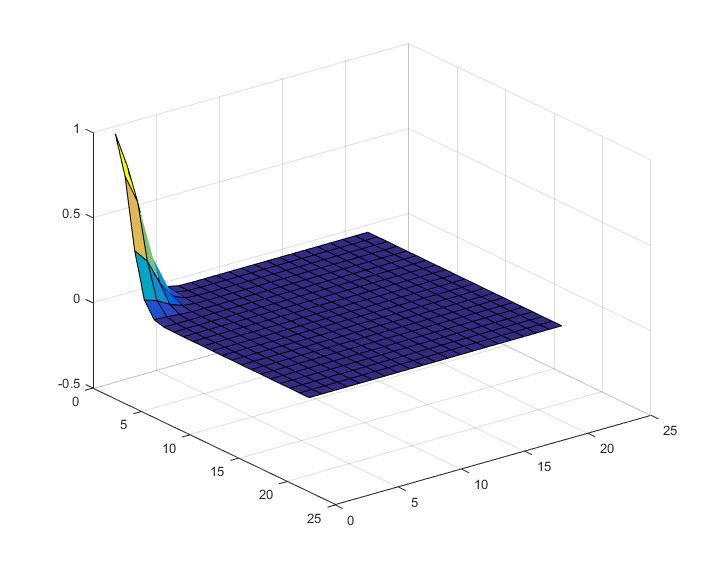
\includegraphics[width=0.2\textwidth]{fig/p2/delt_0p1_del_x_0p05/p2_0.jpg}}
   \subfloat [time=33.3 sec]{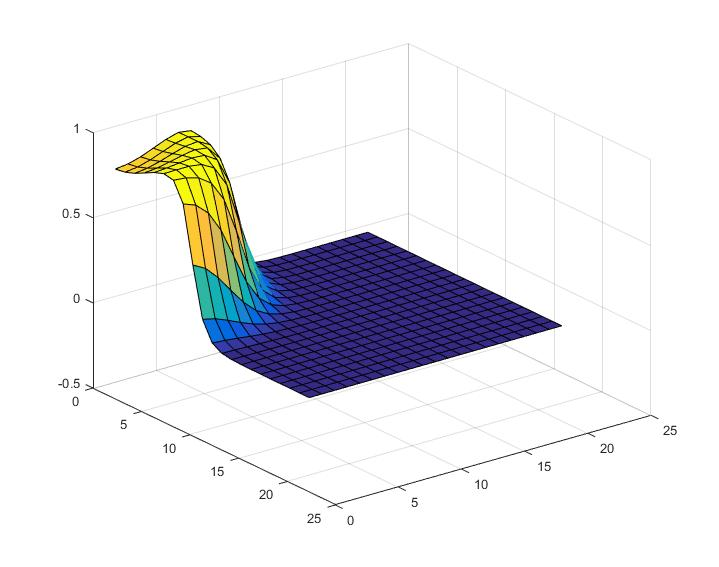
\includegraphics[width=0.2\textwidth]{fig/p2/delt_0p1_del_x_0p05/p2_33p3.jpg}}
   \subfloat [time=66.5 sec]{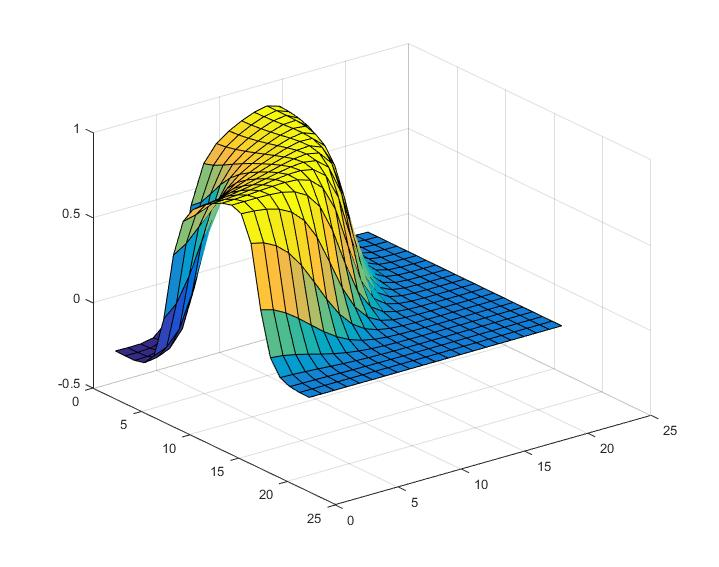
\includegraphics[width=0.2\textwidth]{fig/p2/delt_0p1_del_x_0p05/p2_66p6.jpg}}
   \subfloat [time=99.9 sec]{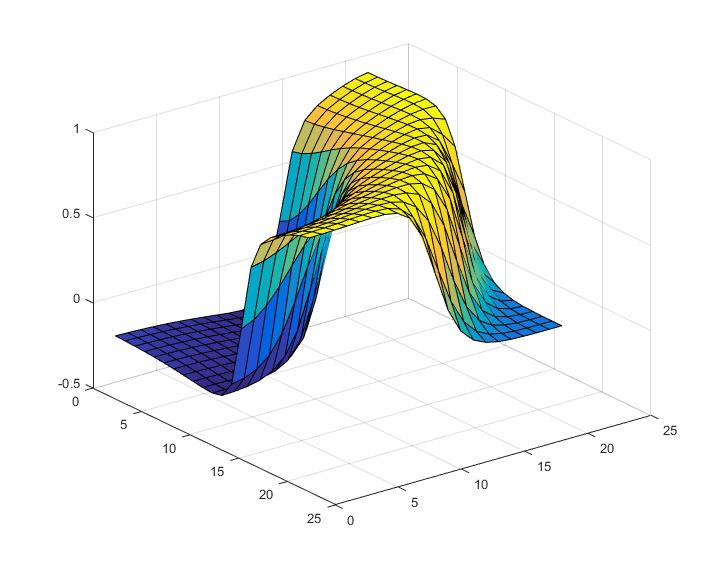
\includegraphics[width=0.2\textwidth]{fig/p2/delt_0p1_del_x_0p05/p2_99p9.jpg}}
   \subfloat [time=133.2 sec]{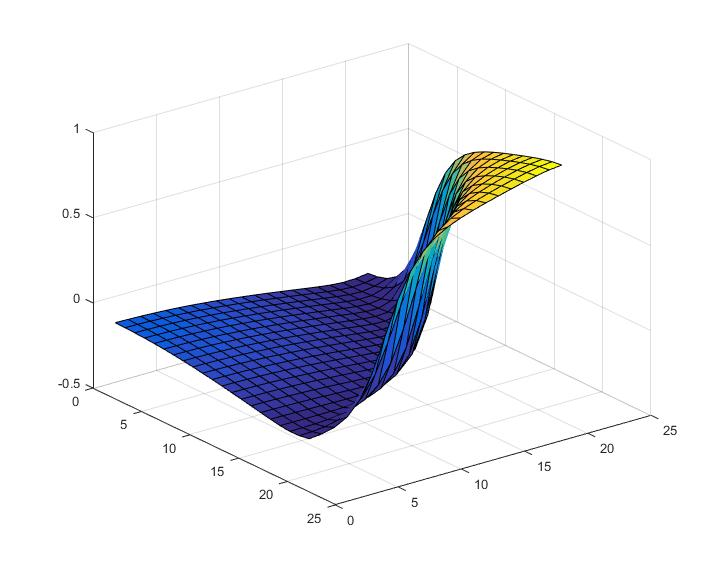
\includegraphics[width=0.2\textwidth]{fig/p2/delt_0p1_del_x_0p05/p2_133p2.jpg}}
   
   \subfloat [time=166.5 sec]{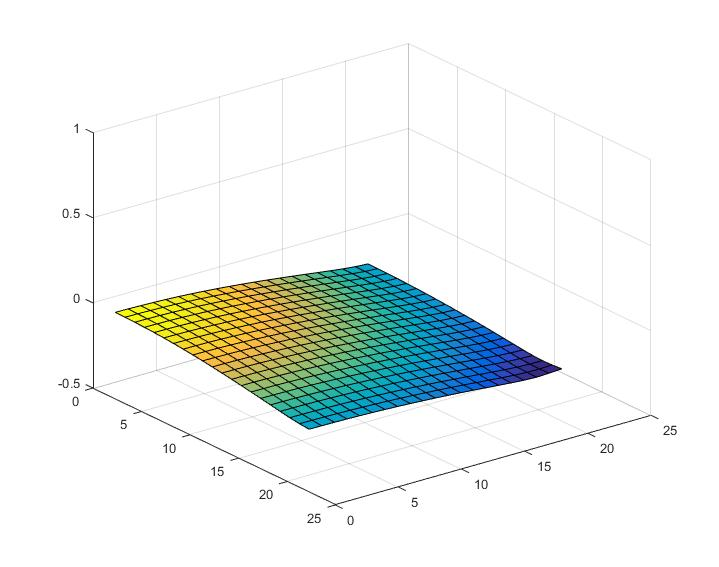
\includegraphics[width=0.2\textwidth]{fig/p2/delt_0p1_del_x_0p05/p2_166p5.jpg}}
   \subfloat [time=199.8 sec]{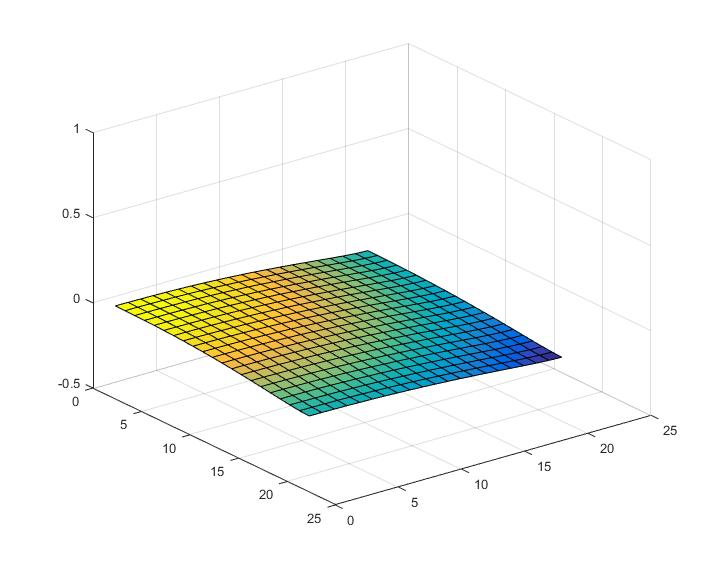
\includegraphics[width=0.2\textwidth]{fig/p2/delt_0p1_del_x_0p05/p2_199p8.jpg}}
   \subfloat [time=233.1 sec]{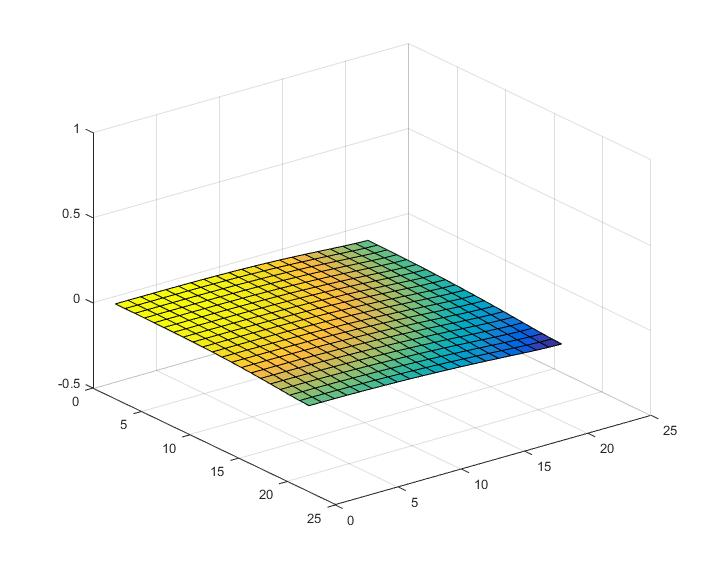
\includegraphics[width=0.2\textwidth]{fig/p2/delt_0p1_del_x_0p05/p2_233p1.jpg}}
   \subfloat [time=266.4 sec]{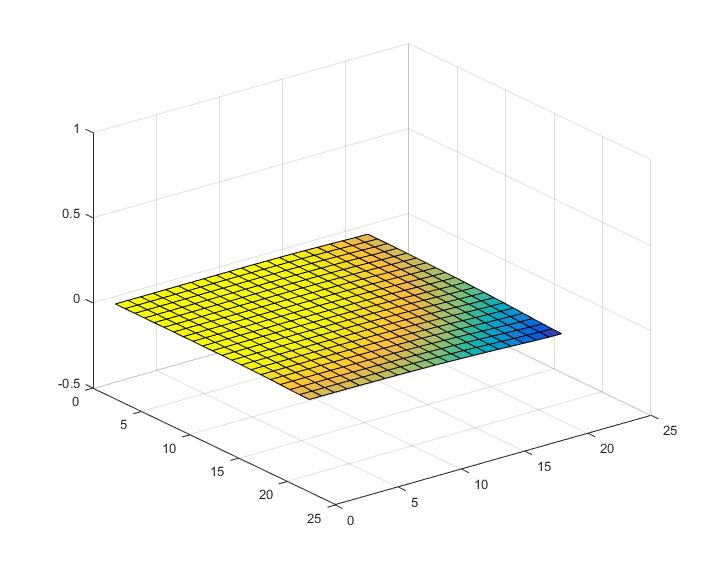
\includegraphics[width=0.2\textwidth]{fig/p2/delt_0p1_del_x_0p05/p2_266p4.jpg}}
   \subfloat [time=299.7 sec]{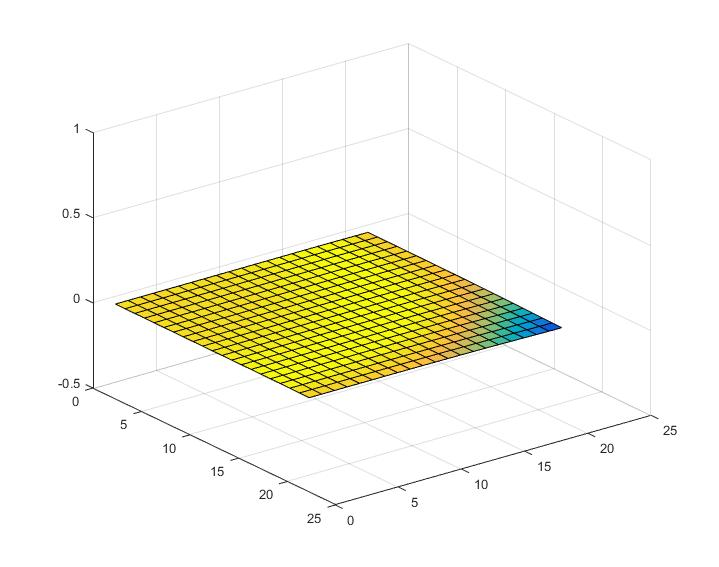
\includegraphics[width=0.2\textwidth]{fig/p2/delt_0p1_del_x_0p05/p2_299p7.jpg}}
   
  \caption{Solution of FirzHugh-Nagumo equations with time and space of $\Delta t=0.1, \Delta x = \Delta y=0.05$ using Strang splitting and ADI for diffusion and RK4 for reaction and $w$ and initial conditions as described in Part 2 and Neumann boundary conditions.}
   \label{fig:sol1}
\end{figure} 
\

\paragraph{Part 3:}
Here we solve the same equation using the same system of equations and solvers but with different initial conditions and up to 600 seconds. The solution is shown in Figure \ref{fig:sol3}. 


\begin{figure}[!tbh]
 \centering  
   \subfloat [time=0   sec]{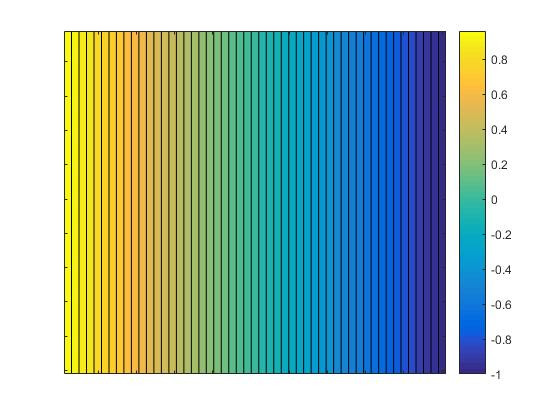
\includegraphics[width=0.2\textwidth]{fig/p2/part3/p2_0.jpg}}
   \subfloat [time=30  sec]{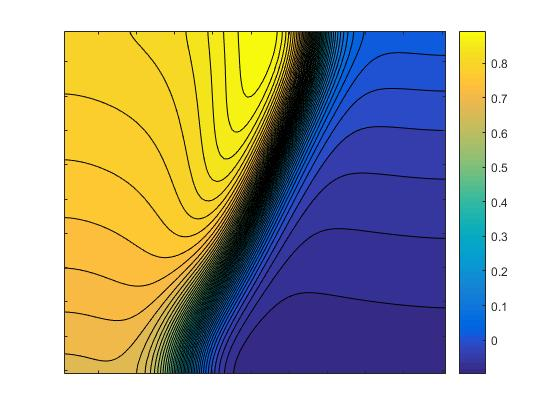
\includegraphics[width=0.2\textwidth]{fig/p2/part3/p2_30p0.jpg}}
   \subfloat [time=60  sec]{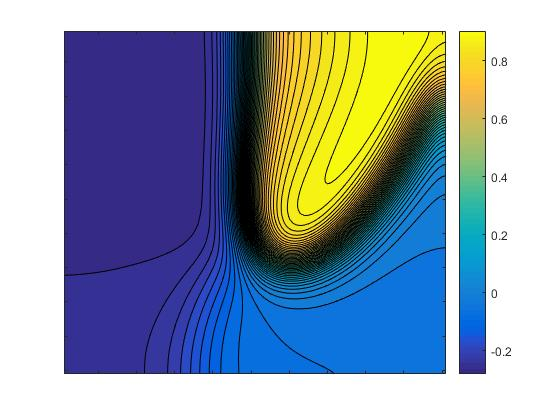
\includegraphics[width=0.2\textwidth]{fig/p2/part3/p2_60p0.jpg}}
   \subfloat [time=90  sec]{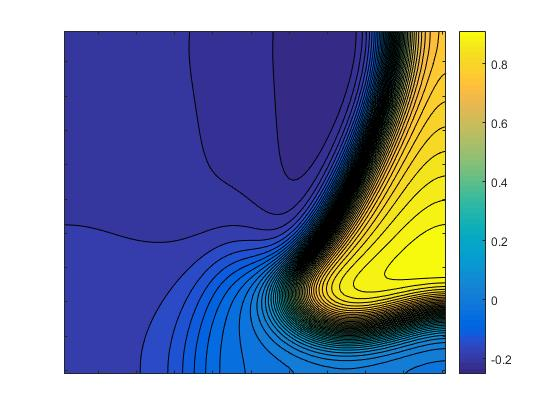
\includegraphics[width=0.2\textwidth]{fig/p2/part3/p2_90p0.jpg}}
   \subfloat [time=120 sec]{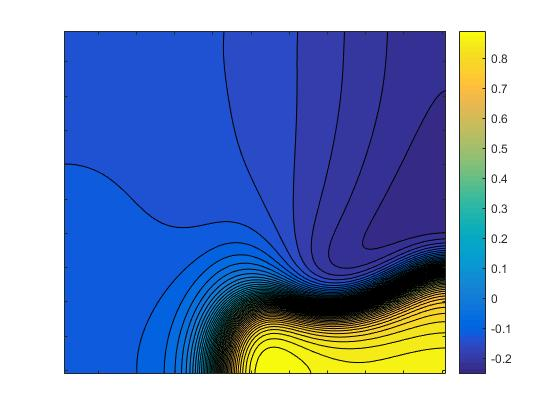
\includegraphics[width=0.2\textwidth]{fig/p2/part3/p2_120p0.jpg}}  
   
   \subfloat [time=150 sec]{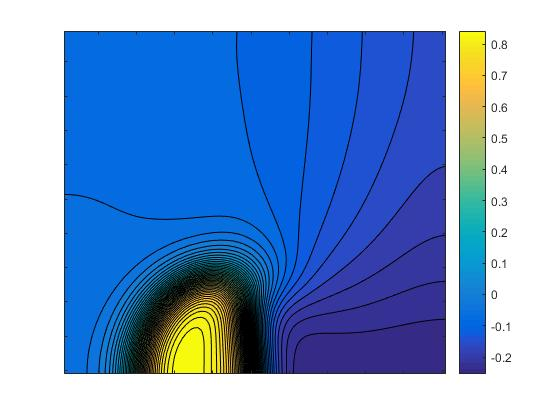
\includegraphics[width=0.2\textwidth]{fig/p2/part3/p2_150p0.jpg}}
   \subfloat [time=180 sec]{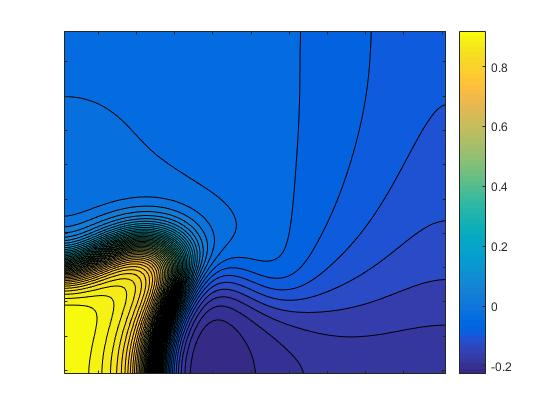
\includegraphics[width=0.2\textwidth]{fig/p2/part3/p2_180p0.jpg}}
   \subfloat [time=210 sec]{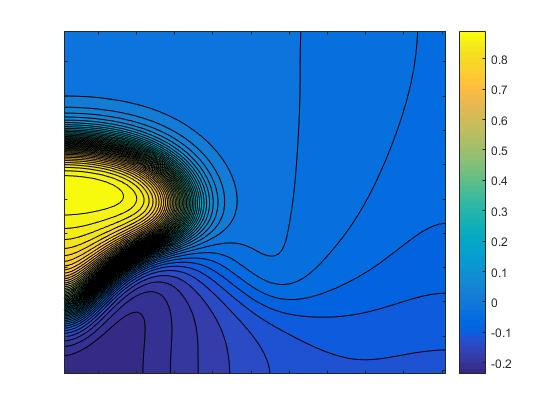
\includegraphics[width=0.2\textwidth]{fig/p2/part3/p2_210p0.jpg}}
   \subfloat [time=240 sec]{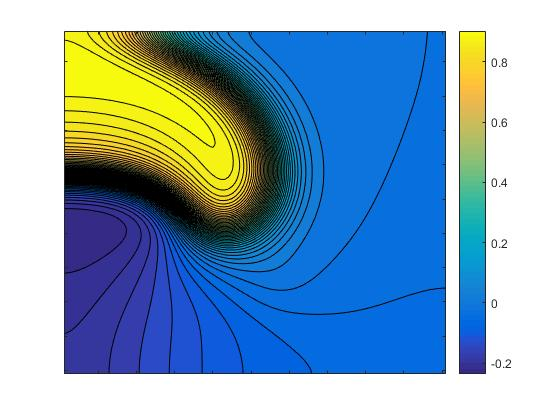
\includegraphics[width=0.2\textwidth]{fig/p2/part3/p2_240p0.jpg}}
   \subfloat [time=270 sec]{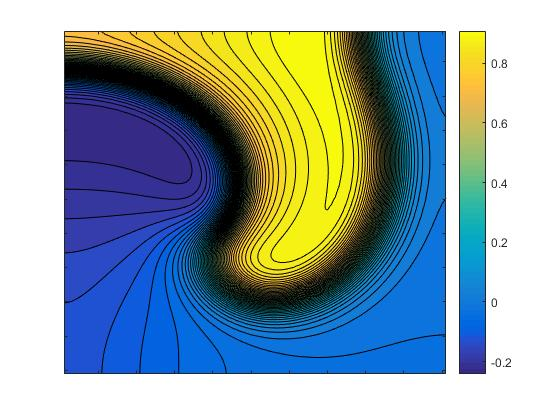
\includegraphics[width=0.2\textwidth]{fig/p2/part3/p2_270p0.jpg}}  
   
   \subfloat [time=300 sec]{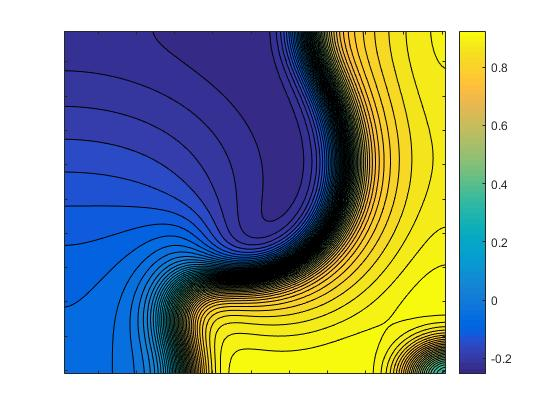
\includegraphics[width=0.2\textwidth]{fig/p2/part3/p2_300p0.jpg}}
   \subfloat [time=330 sec]{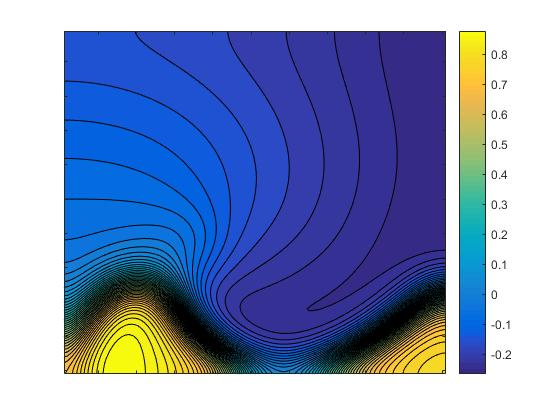
\includegraphics[width=0.2\textwidth]{fig/p2/part3/p2_330p0.jpg}}
   \subfloat [time=360 sec]{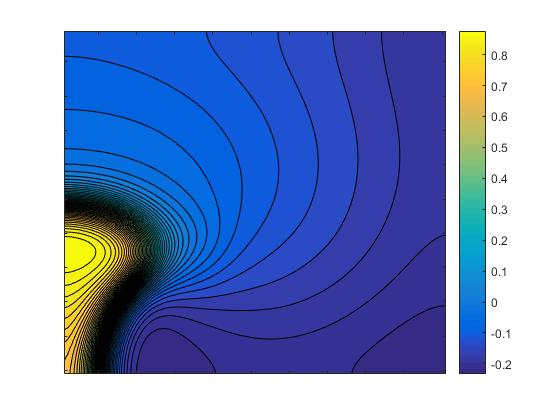
\includegraphics[width=0.2\textwidth]{fig/p2/part3/p2_360p0.jpg}}
   \subfloat [time=390 sec]{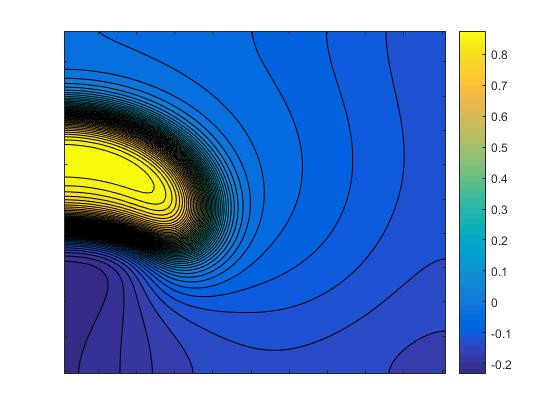
\includegraphics[width=0.2\textwidth]{fig/p2/part3/p2_390p0.jpg}}
   \subfloat [time=420 sec]{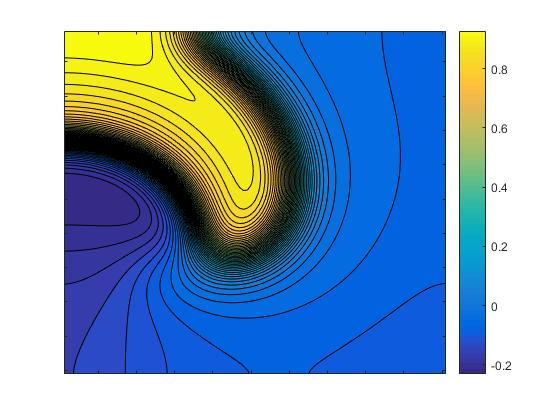
\includegraphics[width=0.2\textwidth]{fig/p2/part3/p2_420p0.jpg}}
   
   \subfloat [time=450 sec]{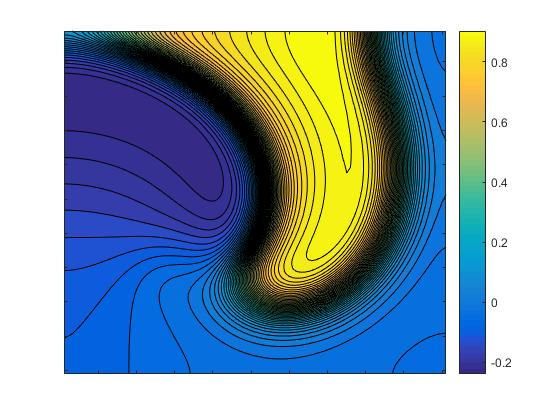
\includegraphics[width=0.2\textwidth]{fig/p2/part3/p2_450p0.jpg}}
   \subfloat [time=480 sec]{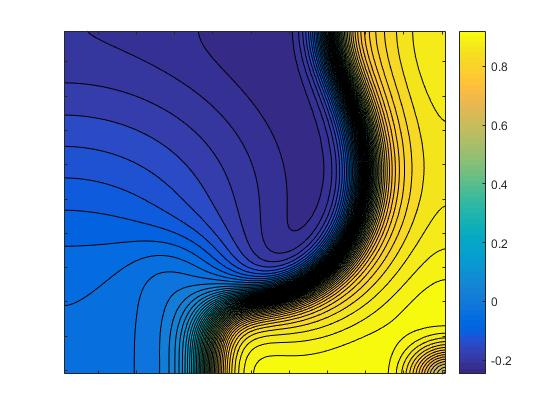
\includegraphics[width=0.2\textwidth]{fig/p2/part3/p2_480p0.jpg}}
   \subfloat [time=510 sec]{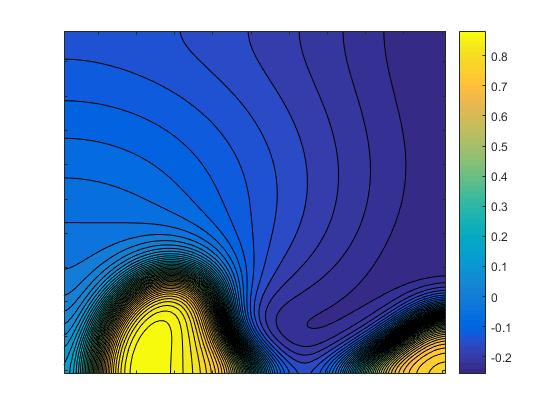
\includegraphics[width=0.2\textwidth]{fig/p2/part3/p2_510p0.jpg}}
   \subfloat [time=540 sec]{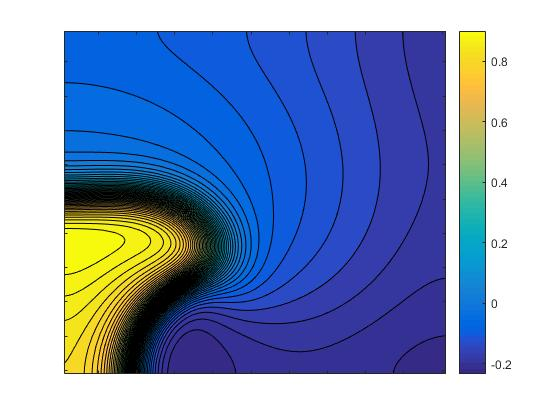
\includegraphics[width=0.2\textwidth]{fig/p2/part3/p2_540p0.jpg}}
   \subfloat [time=600 sec]{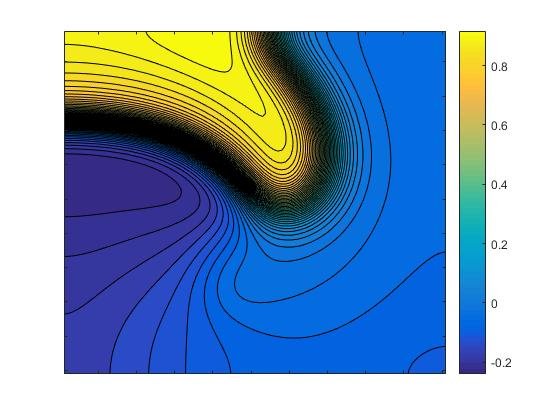
\includegraphics[width=0.2\textwidth]{fig/p2/part3/p2_600p0.jpg}}
 
   
  \caption{Solution of FirzHugh-Nagumo equations with time and space of $\Delta t=0.1, \Delta x = \Delta y=0.05$ using Strang splitting and ADI for diffusion and RK4 for reaction and $w$ and initial conditions as described in Part 3 and Neumann boundary conditions.}
   \label{fig:sol3}
\end{figure} 

With this initial conditions, the voltage represents a linear ramp function from [-1,1]. As the solution advances in time, the initial conditions turns into a spiral-like shape which seems to continue till the end of the simulation time (600 seconds). 

We can see that both the first and second simulations share the phenomena of turning the initial conditions into wave-like shape that spreads across the domain. However, they differ in that the first was able to vanish the effects of the initial conditions and turn to back to rest state. 

